% !TEX root = demo.tex
\section{System Architecture}

In this section, we provide a brief overview of the \sys system and its APIs.
Figure~\ref{fig:arch} depicts the system architecture.

\begin{figure}[t]
\centering
%\vspace{-0.5cm}
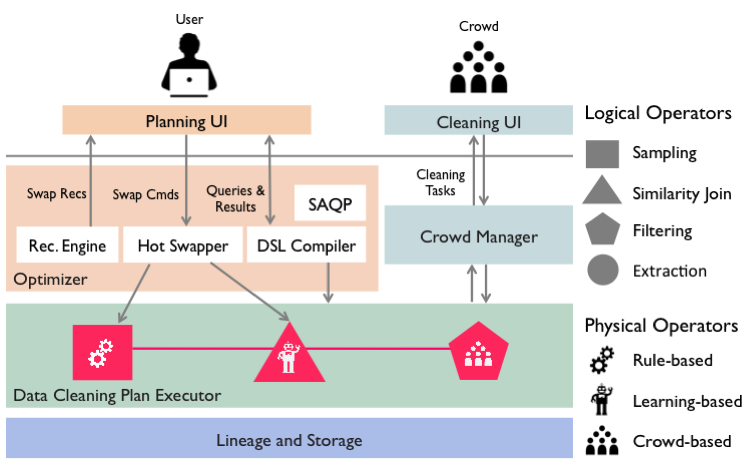
\includegraphics[width = .5\textwidth]{figs/architecture.png}
\vspace{-0.6cm}
\caption{\sys system architecture, with an example entity resolution plan.}
\vspace{-0.3cm}
\label{fig:arch}
\end{figure}

\subsection{Architecture Overview}
The \sys architecture provides UI, language, and systems tools for building data cleaning plans.
Users interact with the system through the \textbf{Planning UI}, which allows them to compose data cleaning workflows from modular operators.
These workflows are represented as expressions in our data cleaning language (section~\ref{sec:dsl}), then synthesized as data cleaning plans by our \textbf{DSL compiler}.
As the \textbf{Data Cleaning Plan Executor} executes the compiled plans, users can interact with the plans via tight feedback loops in two ways.
First, users can issue queries to the Sampling-based Approximate Query Processing \textbf{(SAQP) module} and observe approximate results based on the data that has been cleaned thus far.
Second, the \textbf{Recommendation Engine} displays a set of suggested modifications to the active cleaning plan (for example, making a similarity join more permissive) in the \textbf{Planning UI}, and users can update the data cleaning plan in-flight by accepting a suggestion and using the \textbf{Hot Swapper} to modify components of the pipeline.
Intermediate results and cleaned data are maintained in a \textbf{Lineage and Storage engine} that tracks each tuple's lineage in order to enforce the semantics of hot-swapping correctly on in-flight tuples.
Logical cleaning operators may have a number of physical implementations (section~\ref{sec:operators}).
Automated rule-based or learning-based operators leverage Spark and MLLib for efficient distributed computation, and operators that require human intervention call out to \sys's \textbf{Crowd Manager} API, which renders and displays data cleaning tasks to crowd workers from multiple crowds (e.g., Amazon Mechanical Turk) in a web-based \textbf{Cleaning UI} for processing.

\subsection{Cleaning DSL}
\label{sec:dsl}
We provide a language for specifying the composition of data cleaning operators.
The logical operators define the input and output behavior of the operation and 
the physical operators specify the implementation.
The general syntax of this language is:

{\scriptsize
\begin{lstlisting}
<logical operator> on <relations>
  with <physical operators> , <params>
\end{lstlisting}
}

These expressions are composable. For example, the following represents the cleaning plan in Figure~\ref{fig:arch} (an entity resolution plan):
{\scriptsize
\begin{lstlisting} 
Filtering on (
    SimilartyJoin on (
        Sampling on BaseTable
        with Uniform)
    with Jaccard, thresh=0.8) 
with CrowdDeduplication, numVotes=3
\end{lstlisting}
}
Additionally, \sys provides integration of our DSL with Scala/Apache Spark, allowing DataFrames (Spark RDDs with additional schema information) to serve as base tables in expressions.

\subsection{Cleaning Operators}
\label{sec:operators}
\sys supports a small set of operators that can express a wide variety of common data cleaning workflows. 
For example, the pipeline depicted in Figure~\ref{fig:arch} performs crowd-based entity resolution: the \textsf{SimilarityJoin} operator generates candidate tuple pairs (the \textit{blocking} step), and the crowd-based \textsf{Filter} operator uses humans to identify duplicates from the candidates (the \textit{matching} step). 
Additional operators include Extraction and Sampling.

Individual logical operators have multiple physical implementations, each with its own cost, latency, and accuracy profile. 
For example, crowd-based implementations tend to be high cost, high latency, and high accuracy, whereas rule-based implementations tend to be low cost, low latency, and low accuracy. 
The \texttt{with} clause of our data cleaning language allows users to explicitly specify physical operators, and \sys's recommendation engine suggests pipeline modifications to navigate the tradeoff space.





